\chapter{Amina dan Senyawa Nitrogen}\label{ch:b2:amines}

Ikan yang sudah tidak segar berbau trimetilamina, sebuah amina kecil yang
mudah menguap. Perasan jeruk nipis menghilangkan bau itu: asamnya
memprotonasi amina, dan ion amonium yang terbentuk, karena merupakan ion,
tidak dapat menguap. Pasangan elektron bebas nitrogen membuat amina menjadi
basa dan nukleofil; jika terikat pada karbonil, pasangan itu menghasilkan
\omterm{def:b2:amines:imine}{imina}, yang melaluinya protein menjalankan kimianya dan kimiawan membuat
amina; dan pada cincin \omterm{def:b2:huckel:aromatic}{aromatik}, melalui garam diazonium, pasangan itu
membuka jalan menuju zat warna azo yang mewarnai abad kesembilan belas.

\begin{recall}
Jilid Tahun 1: asam dan basa Brønsted, $\mathrm pK_a$ dan diagram predominansi,
nukleofil dan substitusi bimolekular, hemiasetal dan asetal, donor hidrida,
pereaksi organomagnesium, kelas sebuah karbon. \Cref{ch:b2:aromatic-substitution}:
nitrasi, reduksi nitroarena. Jilid sekolah: amina dan amida.
\end{recall}

\begin{omfigure}
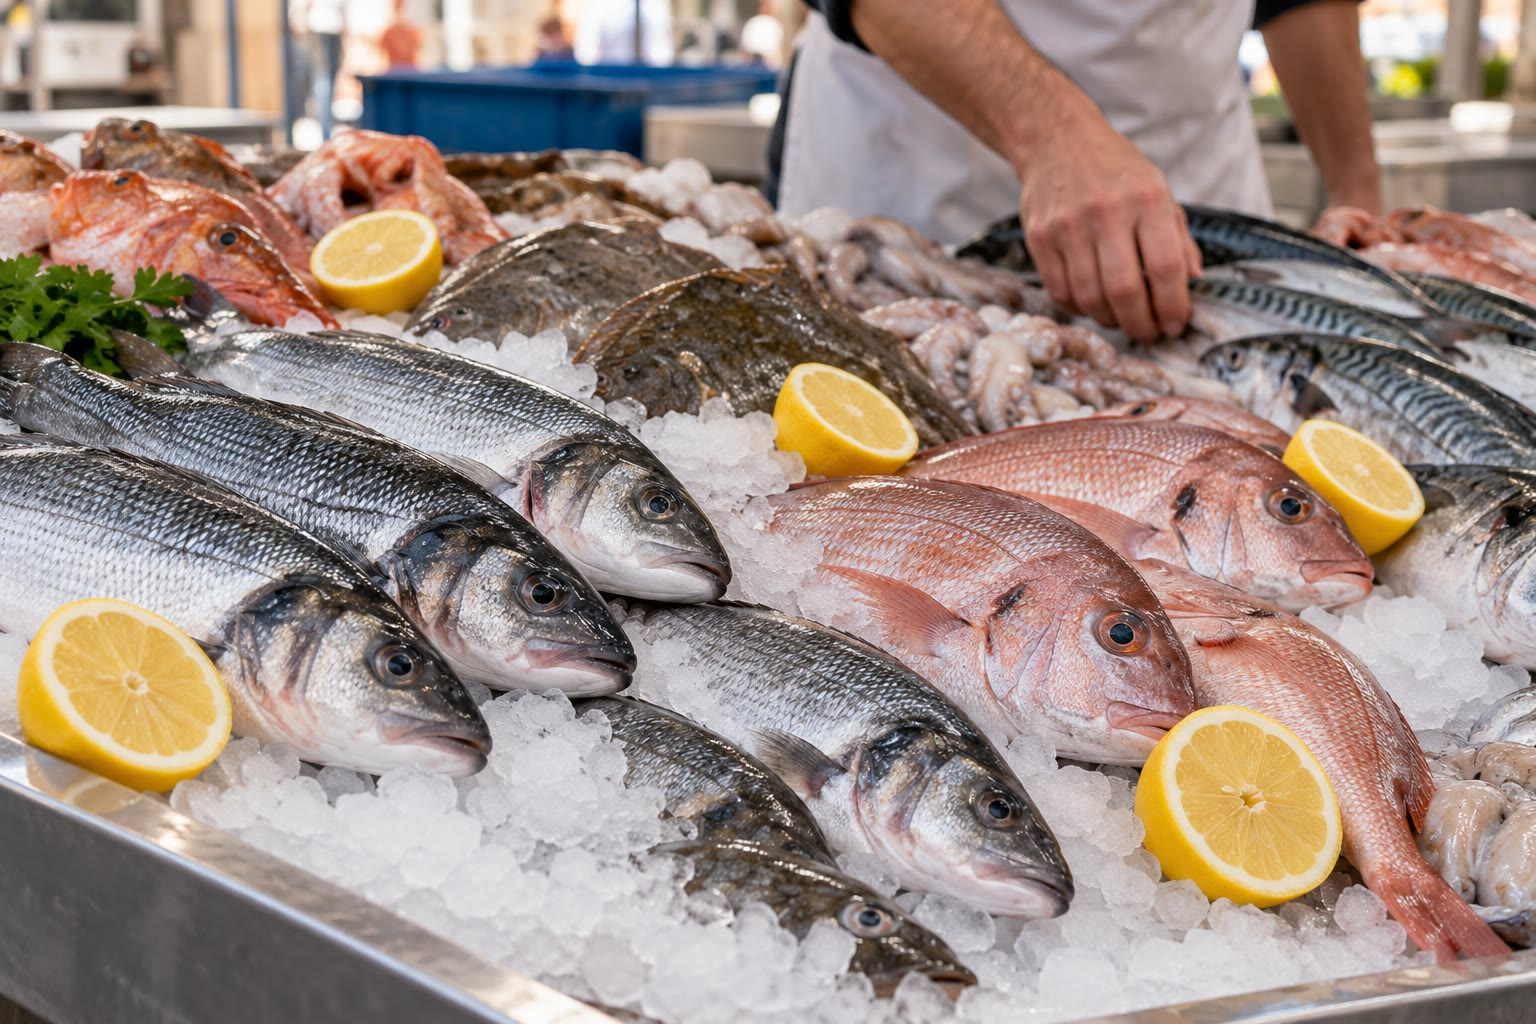
\includegraphics[width=0.6\linewidth]{images/book3/ai/b2-23-fish-stall.jpg}

{\small Sebuah lapak ikan: potongan-potongan jeruk nipis diletakkan di antara
ikan-ikan. Asamnya mengubah trimetilamina ikan menjadi ion amoniumnya yang
tidak mudah menguap.}
\end{omfigure}

\section{Struktur dan kebasaan}

\begin{definition}[Kelas amina]\label{def:b2:amines:class}
Sebuah amina adalah \emph{amina primer}\index{amina primer} \ce{RNH2}, \emph{amina sekunder}
\index{amina sekunder} \ce{R2NH}, atau \emph{amina tersier}\index{amina tersier}
\ce{R3N} menurut jumlah gugus karbon yang terikat pada nitrogen. Sebuah
\emph{ion amonium kuaterner}\index{ion amonium kuaterner} \ce{R4N+}
mempunyai empat, dan tidak mempunyai pasangan elektron bebas.
\end{definition}

Nitrogen amina kira-kira tetrahedral, dengan pasangan elektron bebas yang
menempati posisi keempat. \omterm{def:b2:amines:class}{Amina tersier} dengan tiga gugus yang berbeda pada
prinsipnya kiral tetapi tidak dapat dipisahkan menjadi enansiomernya:
molekul itu terinversi melalui susunan planar, seperti payung yang tertiup
angin, ribuan juta kali per detik pada suhu kamar.

\begin{proposition}[Kebasaan]\label{prop:b2:amines:basicity}
Dalam air, alkilamina adalah basa yang lebih kuat daripada amonia
($\mathrm pK_a$ ion-ion amoniumnya sekitar 10 sampai 11, dibandingkan dengan 9.26), arilamina
jauh lebih lemah (anilinium 4.60), dan amida hampir tidak bersifat basa
sama sekali (etanamida terprotonasi sekitar $-0.6$).
\end{proposition}

\begin{proof}[Argumen]
Gugus-gugus alkil mendorong kerapatan elektron ke nitrogen (efek induktif)
dan menstabilkan muatan positif ion amonium. Dalam air, solvasi melalui
ikatan hidrogen juga berperan: ion dengan lebih banyak ikatan \ce{N-H} lebih
baik tersolvasi, itulah sebabnya trimetilamonium (9.80) adalah asam yang
lebih lemah daripada amonium tetapi lebih kuat daripada dimetilamonium
(10.73). Dalam anilina, pasangan elektron bebasnya terdelokalisasi ke dalam
cincin dan hilang pada protonasi; dalam amida, pasangan itu terdelokalisasi
ke oksigen karbonil, dan protonasi terjadi, secara lemah, pada oksigen.
% ledger: kb:NH3, pka:methylammonium, pka:dimethylammonium, pka:trimethylammonium, pka:anilinium, pka:ethanamideH
\end{proof}

\begin{omfigure}
\begin{tikzpicture}[font=\small, x=0.85cm]
  \draw[->, thick] (-1.5,0) -- (11.8,0) node[below right] {$\mathrm pK_a$};
  \foreach \x in {0,2,4,6,8,10} \draw (\x,0.1) -- (\x,-0.1) node[below, font=\scriptsize] {\x};
  \foreach \x/\l in {-0.6/{\ce{CH3CONH3+}}, 4.60/{\ce{C6H5NH3+}}} {
    \draw[omDef, thick] (\x,0) -- (\x,0.5);
    \node[font=\scriptsize, anchor=south] at (\x,0.5) {\l};
  }
  \foreach \x/\l/\y/\h in {9.26/{\ce{NH4+} (9.26)}/1.95/1.2, 9.80/{\ce{(CH3)3NH+} (9.80)}/1.45/0.85, 10.66/{\ce{CH3NH3+} (10.66)}/0.95/0.5, 10.73/{\ce{(CH3)2NH2+} (10.73)}/0.45/0.25} {
    \draw[omDef, thick] (\x,0) -- (\x,\h);
    \draw[black!40] (\x,\h) -- (12.2,\y);
    \node[font=\scriptsize, anchor=west] at (12.2,\y) {\l};
  }
  \node[font=\scriptsize, anchor=north west] at (-1.4,-0.5) {basa lebih lemah};
  \node[font=\scriptsize, anchor=north east] at (11.7,-0.5) {basa lebih kuat};
\end{tikzpicture}

{\small $\mathrm pK_a$ asam konjugasi beberapa basa nitrogen pada
\qty{25}{\degreeCelsius}: makin tinggi nilainya, makin kuat basanya.}
% ledger: kb:NH3, pka:methylammonium, pka:dimethylammonium, pka:trimethylammonium, pka:anilinium, pka:ethanamideH
\end{omfigure}

\section{Amina sebagai nukleofil}

Amina menyerang haloalkana melalui substitusi bimolekular. Produknya, amina
yang lebih tersubstitusi, sekurang-kurangnya sama nukleofiliknya dengan
amina awal dan bersaing memperebutkan haloalkana: alkilasi amonia
menghasilkan campuran \omterm{def:b2:amines:class}{amina primer}, sekunder, dan tersier serta garam
kuaterner.

\begin{proposition}[Polialkilasi]\label{prop:b2:amines:polyalkylation}
Alkilasi langsung amonia atau \omterm{def:b2:amines:class}{amina primer} menghasilkan campuran; hanya
alkilasi tuntas sampai garam amonium kuaterner yang bersih.
\end{proposition}

\begin{proof}[Argumen]
Setiap alkilasi meninggalkan pasangan elektron bebas pada nitrogen yang
menjadi lebih kaya elektron karena gugus alkil yang baru; produknya bereaksi
dengan haloalkana yang tersisa pada laju yang sebanding. Hanya ketika
nitrogen tidak lagi mempunyai pasangan elektron bebas, dalam \ce{R4N+},
urutan itu berhenti.
\end{proof}

\omterm{def:b2:amines:class}{Amina primer} yang bebas dari kerabat-kerabatnya yang teralkilasi berlebih
dibuat secara tidak langsung: melalui jalur Gabriel (alkilasi nitrogen
ftalimida, yang membawa satu hidrogen asam saja, lalu pelepasan aminanya),
melalui reduksi \omterm{def:b2:amines:nitrile}{nitril}, amida, atau senyawa nitro, atau melalui \omterm{def:b2:amines:reductive-amination}{aminasi
reduktif} (di bawah).

\section{Imina dan enamina}

\begin{definition}[Adisi nukleofilik]\label{def:b2:amines:nucleophilic-addition}
Yang disebut \emph{adisi nukleofilik}\index{adisi nukleofilik} pada gugus
karbonil adalah serangan nukleofil pada karbon karbonil, yang menjadi
tetrahedral, sementara ikatan $\pi$ \ce{C=O} menjadi
pasangan elektron bebas pada oksigen.
\end{definition}

\begin{definition}[Hemiaminal, imina, dan enamina]\label{def:b2:amines:imine}
\omterm{def:b2:amines:class}{Amina primer} beradisi pada aldehida atau keton dan menghasilkan
\emph{hemiaminal}\index{hemiaminal} (karbon yang membawa \ce{OH} dan \ce{NHR});
dehidrasinya menghasilkan \emph{imina}\index{imina}
$\mathrm{R_2C{=}NR'}$. \omterm{def:b2:amines:class}{Amina sekunder}, yang tidak dapat membentuk imina netral, setelah
dehidrasi menghasilkan
\emph{enamina}\index{enamina} $\mathrm{R_2C{=}CR{-}NR'_2}$, dengan ikatan
rangkap yang berpindah ke karbon di sebelahnya.
\end{definition}

\begin{omfigure}
\setchemfig{atom sep=1.9em}
\schemestart
\chemfig{R_2C=O} \+ \chemfig{H_2N-R'}
\arrow{<=>}
\chemfig{R_2C(-[2]OH)-NH-R'}
\arrow{<=>[\ce{H+}][$-$ \ce{H2O}]}
\chemfig{R_2C=N-R'}
\schemestop
\par\vspace{6pt}

{\small Pembentukan \omterm{def:b2:amines:imine}{imina}: \omterm{def:b2:amines:nucleophilic-addition}{adisi nukleofilik} amina pada karbonil
menghasilkan \omterm{def:b2:amines:imine}{hemiaminal}; katalisis asam mengubah \ce{OH}-nya menjadi gugus
pergi (\ce{-OH2+}), air pergi, dan pasangan elektron bebas nitrogen
membentuk ikatan rangkap \ce{C=N}. Setiap tahap reversibel: air berlebih
menghidrolisis \omterm{def:b2:amines:imine}{imina} kembali.}
\end{omfigure}

\begin{proposition}[pH optimal]\label{prop:b2:amines:imine-ph}
\omterm{def:b2:amines:imine}{Imina} terbentuk paling cepat dalam larutan yang agak asam, sekitar pH 4 sampai 5.
\end{proposition}

\begin{proof}[Argumen]
Tahap pertama memerlukan amina bebas (pasangan elektron bebasnya); medium
yang terlalu asam memprotonasi amina ($\mathrm pK_a$ sekitar 10) dan
menghilangkan nukleofilnya. Dehidrasi memerlukan asam untuk memprotonasi
gugus hidroksil; pada pH tinggi dehidrasi berjalan lambat. Lajunya, hasil
kali kedua kebutuhan itu, paling besar di antaranya.
\end{proof}

\begin{definition}[Aminasi reduktif]\label{def:b2:amines:reductive-amination}
Yang disebut \emph{aminasi reduktif}\index{aminasi reduktif} mengubah
senyawa karbonil dan amina menjadi amina yang lebih tersubstitusi dengan
membentuk \omterm{def:b2:amines:imine}{imina} (atau ion iminium) dan mereduksinya dalam wadah yang sama,
biasanya dengan natrium sianoborohidrida \ce{NaBH3CN}.
\end{definition}

\begin{proposition}[Selektivitas aminasi reduktif]\label{prop:b2:amines:reductive-amination}
Pada pH sekitar 6, \ce{NaBH3CN} mereduksi ion iminium jauh lebih cepat
daripada senyawa karbonil, sehingga amina terbentuk tanpa mereduksi
aldehida atau keton menjadi alkohol.
\end{proposition}

\begin{proof}[Argumen]
Gugus siano membuat \ce{BH3CN-} menjadi donor hidrida yang lemah, terlalu
lemah untuk karbonil netral tetapi cukup untuk ion iminium yang terprotonasi
dan bermuatan positif, sebuah elektrofil yang jauh lebih baik.
\end{proof}

\section{Garam diazonium}

\begin{definition}[Kimia diazonium]\label{def:b2:amines:diazonium}
Yang disebut \emph{ion diazonium}\index{ion diazonium} adalah kation \ce{R-N+#N}. \emph{Diazotisasi}\index{diazotisasi}
mengubah amina \omterm{def:b2:huckel:aromatic}{aromatik} primer menjadi garam aril diazonium dengan natrium
nitrit dan asam kuat pada
0--\qty{5}{\degreeCelsius}. Dalam \emph{reaksi Sandmeyer}\index{reaksi Sandmeyer},
garam tembaga(I) (\ce{CuCl}, \ce{CuBr}, \ce{CuCN}) menggantikan gugus
diazonium dengan Cl, Br, atau CN sambil melepaskan dinitrogen. Dalam
\emph{kopling azo}\index{kopling azo}, ion diazonium, sebuah elektrofil
lemah, menyerang cincin \omterm{def:b2:huckel:aromatic}{aromatik} yang teraktivasi dan menghasilkan senyawa
azo $\mathrm{Ar{-}N{=}N{-}Ar'}$.
\end{definition}

\begin{proposition}[Kestabilan ion diazonium]\label{prop:b2:amines:diazonium}
Garam aril diazonium dapat disimpan dalam larutan berair yang dingin dan
dipakai; ion alkil diazonium langsung melepaskan dinitrogen.
\end{proposition}

\begin{proof}[Argumen]
Dinitrogen adalah gugus pergi yang sangat baik (molekul yang sangat stabil,
kenaikan entropi yang besar). Untuk gugus alkil, lepasnya \ce{N2}
menyisakan karbokation, atau ion itu langsung diserang oleh air: ion itu
tidak bertahan. Kation aril sangat tidak stabil (orbital $\sigma$ yang
kosong pada bidang cincin, tidak distabilkan oleh sistem $\pi$), dan ikatan
\ce{C-N} ion aril diazonium diperkuat oleh konjugasi dengan cincin: pada
suhu rendah ion itu bertahan; jika dihangatkan, ion itu terurai, dengan air
yang menggantikan gugus diazonium dengan \ce{OH}.
\end{proof}

\begin{omfigure}
\begin{tikzpicture}[font=\small, >={Stealth}]
  \node[cyclenode] (d) at (0,0) {\ce{Ar-N2+}};
  \foreach \a/\t/\c in {90/{\ce{Ar-Cl}}/{\ce{CuCl}}, 150/{\ce{Ar-Br}}/{\ce{CuBr}}, 210/{\ce{Ar-CN}}/{\ce{CuCN}},
                        270/{\ce{Ar-OH}}/{\ce{H2O}, hangat}, 330/{\ce{Ar-H}}/{\ce{H3PO2}}, 30/{$\mathrm{Ar{-}N{=}N{-}Ar'}$}/{\ce{ArH} teraktivasi}} {
    \node[cyclenode] (p\a) at (\a:2.6) {\t};
    \draw[->, thick] (d) -- (p\a) node[midway, font=\scriptsize, fill=white, inner sep=1pt] {\c};
  }
\end{tikzpicture}

{\small Reaksi-reaksi garam aril diazonium. Gugus \ce{N2+} digantikan oleh
halogen atau sianida (Sandmeyer, garam tembaga(I)), oleh \ce{OH} (air
hangat), atau oleh H (asam hipofosfit), atau dipertahankan dalam \omterm{def:b2:amines:diazonium}{kopling
azo}.}
\end{omfigure}

\begin{method}[Jalur melalui garam diazonium]\label{met:b2:amines:diazonium-routes}
\begin{enumerate}
  \item Pakailah gugus amino (\omterm{def:b2:aromatic-substitution:directing}{pengarah orto/para} yang kuat) untuk
        menempatkan gugus-gugus lain, lalu ubahlah gugus itu melalui garam
        diazonium.
  \item Gantilah gugus itu dengan H untuk memperoleh pola yang tidak dapat
        diberikan oleh substitusi langsung (1,3,5-tribromobenzena dari anilina).
  \item Gantilah gugus itu dengan CN, lalu hidrolisis menjadi asam
        karboksilat: sebuah jalan menuju \ce{-COOH} pada cincin.
\end{enumerate}
\end{method}

\begin{method}[Membuat amina]\label{met:b2:amines:make-amine}
\begin{enumerate}
  \item \omterm{def:b2:amines:class}{Amina primer} pada rantai alkil: jalur Gabriel, atau reduksi \omterm{def:b2:amines:nitrile}{nitril}
        (satu karbon lebih banyak daripada haloalkana yang dipakai untuk
        membuatnya) atau amida.
  \item \omterm{def:b2:amines:class}{Amina sekunder} atau tersier: \omterm{def:b2:amines:reductive-amination}{aminasi reduktif} senyawa karbonil yang
        tepat dengan amina yang tepat.
  \item Amina \omterm{def:b2:huckel:aromatic}{aromatik}: nitrasi, lalu reduksi (besi atau timah dengan asam,
        atau \omterm{def:b2:alkene-redox:hydrogenation}{hidrogenasi katalitik}).
\end{enumerate}
\end{method}

\section{Nitril}

\begin{definition}[Nitril]\label{def:b2:amines:nitrile}
Yang disebut \emph{nitril}\index{nitril} adalah senyawa \ce{R-C#N}, yang
dibuat melalui substitusi haloalkana oleh sianida atau melalui \omterm{def:b2:amines:diazonium}{reaksi
Sandmeyer}.
\end{definition}

\begin{proposition}[Reaksi-reaksi nitril]\label{prop:b2:amines:nitrile}
\omterm{def:b2:amines:nitrile}{Nitril} dihidrolisis, dalam asam atau dalam basa, menjadi amida lalu menjadi
asam karboksilat; \omterm{def:b2:amines:nitrile}{nitril} direduksi oleh litium aluminium hidrida menjadi
\omterm{def:b2:amines:class}{amina primer} \ce{RCH2NH2}; pereaksi organomagnesium beradisi sekali padanya,
dan hidrolisis \omterm{def:b2:amines:imine}{imina} yang terbentuk menghasilkan keton.
\end{proposition}

\begin{proof}[Argumen]
Karbon \omterm{def:b2:amines:nitrile}{nitril} bersifat elektrofilik, seperti karbon karbonil: air
(diaktifkan oleh asam, atau sebagai hidroksida) beradisi padanya, dan
setelah tautomerisasi menghasilkan amida, yang hidrolisisnya dibahas pada
\cref{ch:b2:acyl-substitution}. Hidrida beradisi dua kali. Pereaksi
organomagnesium beradisi sekali dan menghasilkan anion \omterm{def:b2:amines:imine}{imina} yang tidak
bereaksi lebih lanjut; air lalu menghidrolisis \omterm{def:b2:amines:imine}{imina} itu menjadi keton.
\end{proof}

\begin{safety}{\ghs[5mm]{GHS03}\,\ghs[5mm]{GHS06}\,\ghs[5mm]{GHS08}\,\ghs[5mm]{GHS09}}
Anilina dan \textit{N},\textit{N}-dimetilanilina beracun melalui kontak
kulit; natrium nitrit beracun dan bersifat pengoksidasi; natrium
sianoborohidrida melepaskan hidrogen sianida dalam asam dan harus dipakai di
dalam lemari asam. Garam diazonium kering dapat meledak: garam itu selalu
dijaga dingin, dalam larutan, dan langsung dipakai.
% ledger: ghs:aniline, ghs:dimethylaniline, ghs:NaNO2, ghs:NaBH3CN, ghs:sulfanilic-acid
\end{safety}

\section{Latihan}

\begin{exercise}[$\star$]\label{exo:b2:amines:1}
Tentukan kelas: propan-1-amina, \textit{N}-metiletanamina, trietilamina,
tetrametilamonium klorida, anilina.
\end{exercise}

\begin{exercise}[$\star$]\label{exo:b2:amines:2}
Urutkan menurut kebasaan yang meningkat: amonia, metilamina, anilina, etanamida.
\end{exercise}

\begin{exercise}[$\star$]\label{exo:b2:amines:3}
Tuliskan \omterm{def:b2:amines:imine}{imina} yang terbentuk dari sikloheksanon dan metilamina, beserta kondisinya.
\end{exercise}

\begin{exercise}[$\star$]\label{exo:b2:amines:4}
Berawal dari benzenadiazonium klorida, tuliskan produk-produknya dengan
\ce{CuBr}, \ce{CuCN}, air hangat, dan fenol dalam basa.
\end{exercise}

\begin{exercise}[$\star\star$]\label{exo:b2:amines:5}
Bentuk trimetilamina manakah yang dominan pada pH 7, dan dengan rasio
berapa? Jelaskan peran jeruk nipis, dan bagaimana sebuah amina dapat
diekstraksi dari pelarut organik ke dalam air.
\end{exercise}

\begin{exercise}[$\star\star$]\label{exo:b2:amines:6}
Tuliskan \omterm{def:b2:amines:imine}{enamina} yang terbentuk dari sikloheksanon dan pirolidina, dan
jelaskan mengapa \omterm{def:b2:amines:class}{amina sekunder} tidak dapat menghasilkan \omterm{def:b2:amines:imine}{imina}.
\end{exercise}

\begin{exercise}[$\star\star$]\label{exo:b2:amines:7}
Buatlah \textit{N}-benzilpropan-2-amina \ce{C6H5CH2NHCH(CH3)2} melalui
\omterm{def:b2:amines:reductive-amination}{aminasi reduktif}: berikan dua pasangan pereaksi yang mungkin.
\end{exercise}

\begin{exercise}[$\star\star$]\label{exo:b2:amines:8}
Benzonitril bereaksi dengan etilmagnesium bromida, lalu dengan asam berair. Tuliskan produknya.
\end{exercise}

\begin{exercise}[$\star\star$]\label{exo:b2:amines:9}
Tuliskan sintesis Gabriel heksan-1-amina dan jelaskan mengapa sintesis itu tidak menghasilkan \omterm{def:b2:amines:class}{amina sekunder}.
\end{exercise}

\begin{exercise}[$\star\star\star$]\label{exo:b2:amines:10}
Buatlah 1,3,5-tribromobenzena dari anilina.
\end{exercise}

\begin{exercise}[$\star\star\star$]\label{exo:b2:amines:11}
Rancanglah sebuah zat warna azo dari 4-nitroanilina dan fenol: tuliskan
\omterm{def:b2:amines:diazonium}{diazotisasinya}, koplingnya (posisi dan pH), dan produknya.
\end{exercise}

\begin{exercise}[$\star\star\star$]\label{exo:b2:amines:12}
Hidroksida amonium kuaterner dari \textit{N},\textit{N}-dimetilbutan-2-amina,
jika dipanaskan, terutama menghasilkan but-1-ena. Jelaskan orientasi Hofmann
ini, yang berlawanan dengan aturan Zaitsev dari jilid Tahun 1.
\end{exercise}

\section{Soal: Membuat Metil Jingga}

\begin{problem}[{Soal akhir pekan --- asam sulfanilat dan \omterm{def:b2:amines:diazonium}{diazotisasinya},
\omterm{def:b2:amines:diazonium}{kopling azo} dengan \textit{N},\textit{N}-dimetilanilina, metil jingga sebagai
indikator, dan rendemennya}]
\label{pb:b2:amines:1}
Data: asam sulfanilat (asam 4-aminobenzenasulfonat) \ce{C6H7NO3S}; metil
jingga, garam natriumnya
\ce{C14H14N3NaO3S}; $\mathrm pK_a$ bentuk asam metil jingga 3.47. Massa molar
(\unit{g/mol}): C 12.011, H 1.008, N 14.007, O 15.999, Na 22.990, S 32.06.
Percobaan (data latihan): \qty{5.00}{g} asam sulfanilat, rendemen 80~\%.
% ledger: pka:methylorange, aw:C, aw:H, aw:N, aw:O, aw:Na, aw:S, ghs:sulfanilic-acid, ghs:NaNO2

\medskip
\noindent\textbf{Bagian I --- Asam sulfanilat dan \omterm{def:b2:amines:diazonium}{diazotisasi}.}
\begin{enumerate}
  \item Asam sulfanilat berada sebagai zwitterion. Gambarlah zwitterion itu.
  \item Mengapa asam itu dilarutkan dalam larutan natrium karbonat lebih dahulu?
  \item Tuliskan pembentukan asam nitrit dari natrium nitrit dan asam klorida.
  \item Tuliskan \omterm{def:b2:amines:diazonium}{diazotisasi} ion 4-sulfonatoanilinium.
  \item Mengapa reaksi itu dijalankan pada 0--\qty{5}{\degreeCelsius}?
  \item Berapa jumlah natrium nitrit yang diperlukan untuk \qty{5.00}{g}
        asam sulfanilat?
  \item Mengapa sedikit kelebihan nitrit diuji, lalu dimusnahkan?
\end{enumerate}

\medskip
\noindent\textbf{Bagian II --- Kopling.}
\begin{enumerate}[resume]
  \item Mengapa \textit{N},\textit{N}-dimetilanilina merupakan pasangan yang baik?
  \item Pada posisi manakah dari cincinnya \omterm{def:b2:amines:diazonium}{ion diazonium} menyerang, dan mengapa?
  \item Tuliskan produknya (sebagai sulfonat).
  \item Mengapa kopling dijalankan dalam larutan yang asam lemah, bukan asam kuat?
  \item Mengapa larutan itu kemudian harus dibuat basa untuk mengendapkan
        garam natriumnya?
  \item Mengapa \omterm{def:b2:amines:diazonium}{ion diazonium} merupakan elektrofil lemah, yang hanya
        bereaksi dengan cincin yang teraktivasi?
\end{enumerate}

\medskip
\noindent\textbf{Bagian III --- Sebuah indikator.}
\begin{enumerate}[resume]
  \item Apa warna metil jingga dalam basa, dan dalam asam?
  \item Di mana metil jingga menerima proton?
  \item Pada rentang pH berapakah warnanya berubah?
  \item Mengapa sistem terkonjugasi yang panjang menghasilkan warna yang tampak?
  \item Mengapa protonasi menggeser serapannya?
\end{enumerate}

\medskip
\noindent\textbf{Bagian IV --- Rendemen.}
\begin{enumerate}[resume]
  \item Hitunglah massa molar asam sulfanilat.
  \item Hitunglah massa molar metil jingga (garam natrium).
  \item Hitunglah jumlah asam sulfanilat yang dipakai.
  \item Hitunglah massa teoretis metil jingga.
  \item Kehilangan apa saja yang menjelaskan rendemen di bawah 100~\%?
  \item Nyatakan massa metil jingga yang diperoleh dari \qty{5.00}{g} asam
        sulfanilat pada rendemen 80~\%.
\end{enumerate}
\end{problem}
